\newpage
\section{Описание разрабатываемой автоматизированной системы коммерческого учета энергоресурсов}
\setcounter{figure}{0}

Основными  потребителями  электросчетчиков российского производства являются страны СНГ, Украина и Казахстан – лидеры по потреблению в 2007-2013 году (на долю экспорта в эти страны приходится около  80\% [1] ). Для учета использования электроэнергии существуют автоматизированные системы коммерческого учета электроэнергии (АСКУЭ).

Автоматизированная система коммерческого учета энергоресурсов (АСКУЭ) - это программно-аппаратный комплекс, предназначенный для сбора, хранени и обработки инофрмации о потреблении энергоресурсов на объекте. 

Аппаратная часть представлена устройствами учета(УУ), устройствами сбора и передачи данных(УСПД), а так же центральным сервером(ЦС).

Программная часть включает в себя прошивки УУ и УСПД, ПО для ЦС.

ПО ЦС предназначено для сбора показаний с точек учета энергоресурсов, а также архивирования, хранения, анализа и визуализации полученных данных, формирования отчетов. Под показаниями подразумеваются данные о потребляемой мощности электроэнергии потребителями однофазных и трехфазных сетей.

Областью применения ПО ЦС являются объекты жилого, коммерческого и производственного назначения.

ПО ЦС — это программный комплекс, который должен включать в себя сервер баз данных, сервер сбора данных(ССД), сервер приложений, web-сервер, АРМ оператора, АРМ администратора, АРМ клиента, АРМ сервисного инженера(АРМ СИ).

ПО ССД должно выполнять следующие функции:
\begin{itemize}
 \item взаимодействие с УСПД и счетчиками (опрос и сбор данных);
 \item взаимодействие с СБД (запись обработанных данных для дальнейшей работы с ними);
 \item преобразование полученных данных в удобный для дальнейшей обработки формат;
 \item мониторинг и обработка ошибок;
 \item журналирование событий ССД.
\end{itemize}

ПО ЦС представляет собой иерархическую систему сбора, передачи и хранения данных (рис. \ref{irsh:irsh}). Информация от первичных приборов учета посредством УСПД поступает на ССД, который обеспечивает ее обработку и запись на СБД.

\begin{figure}[h!]
 \center{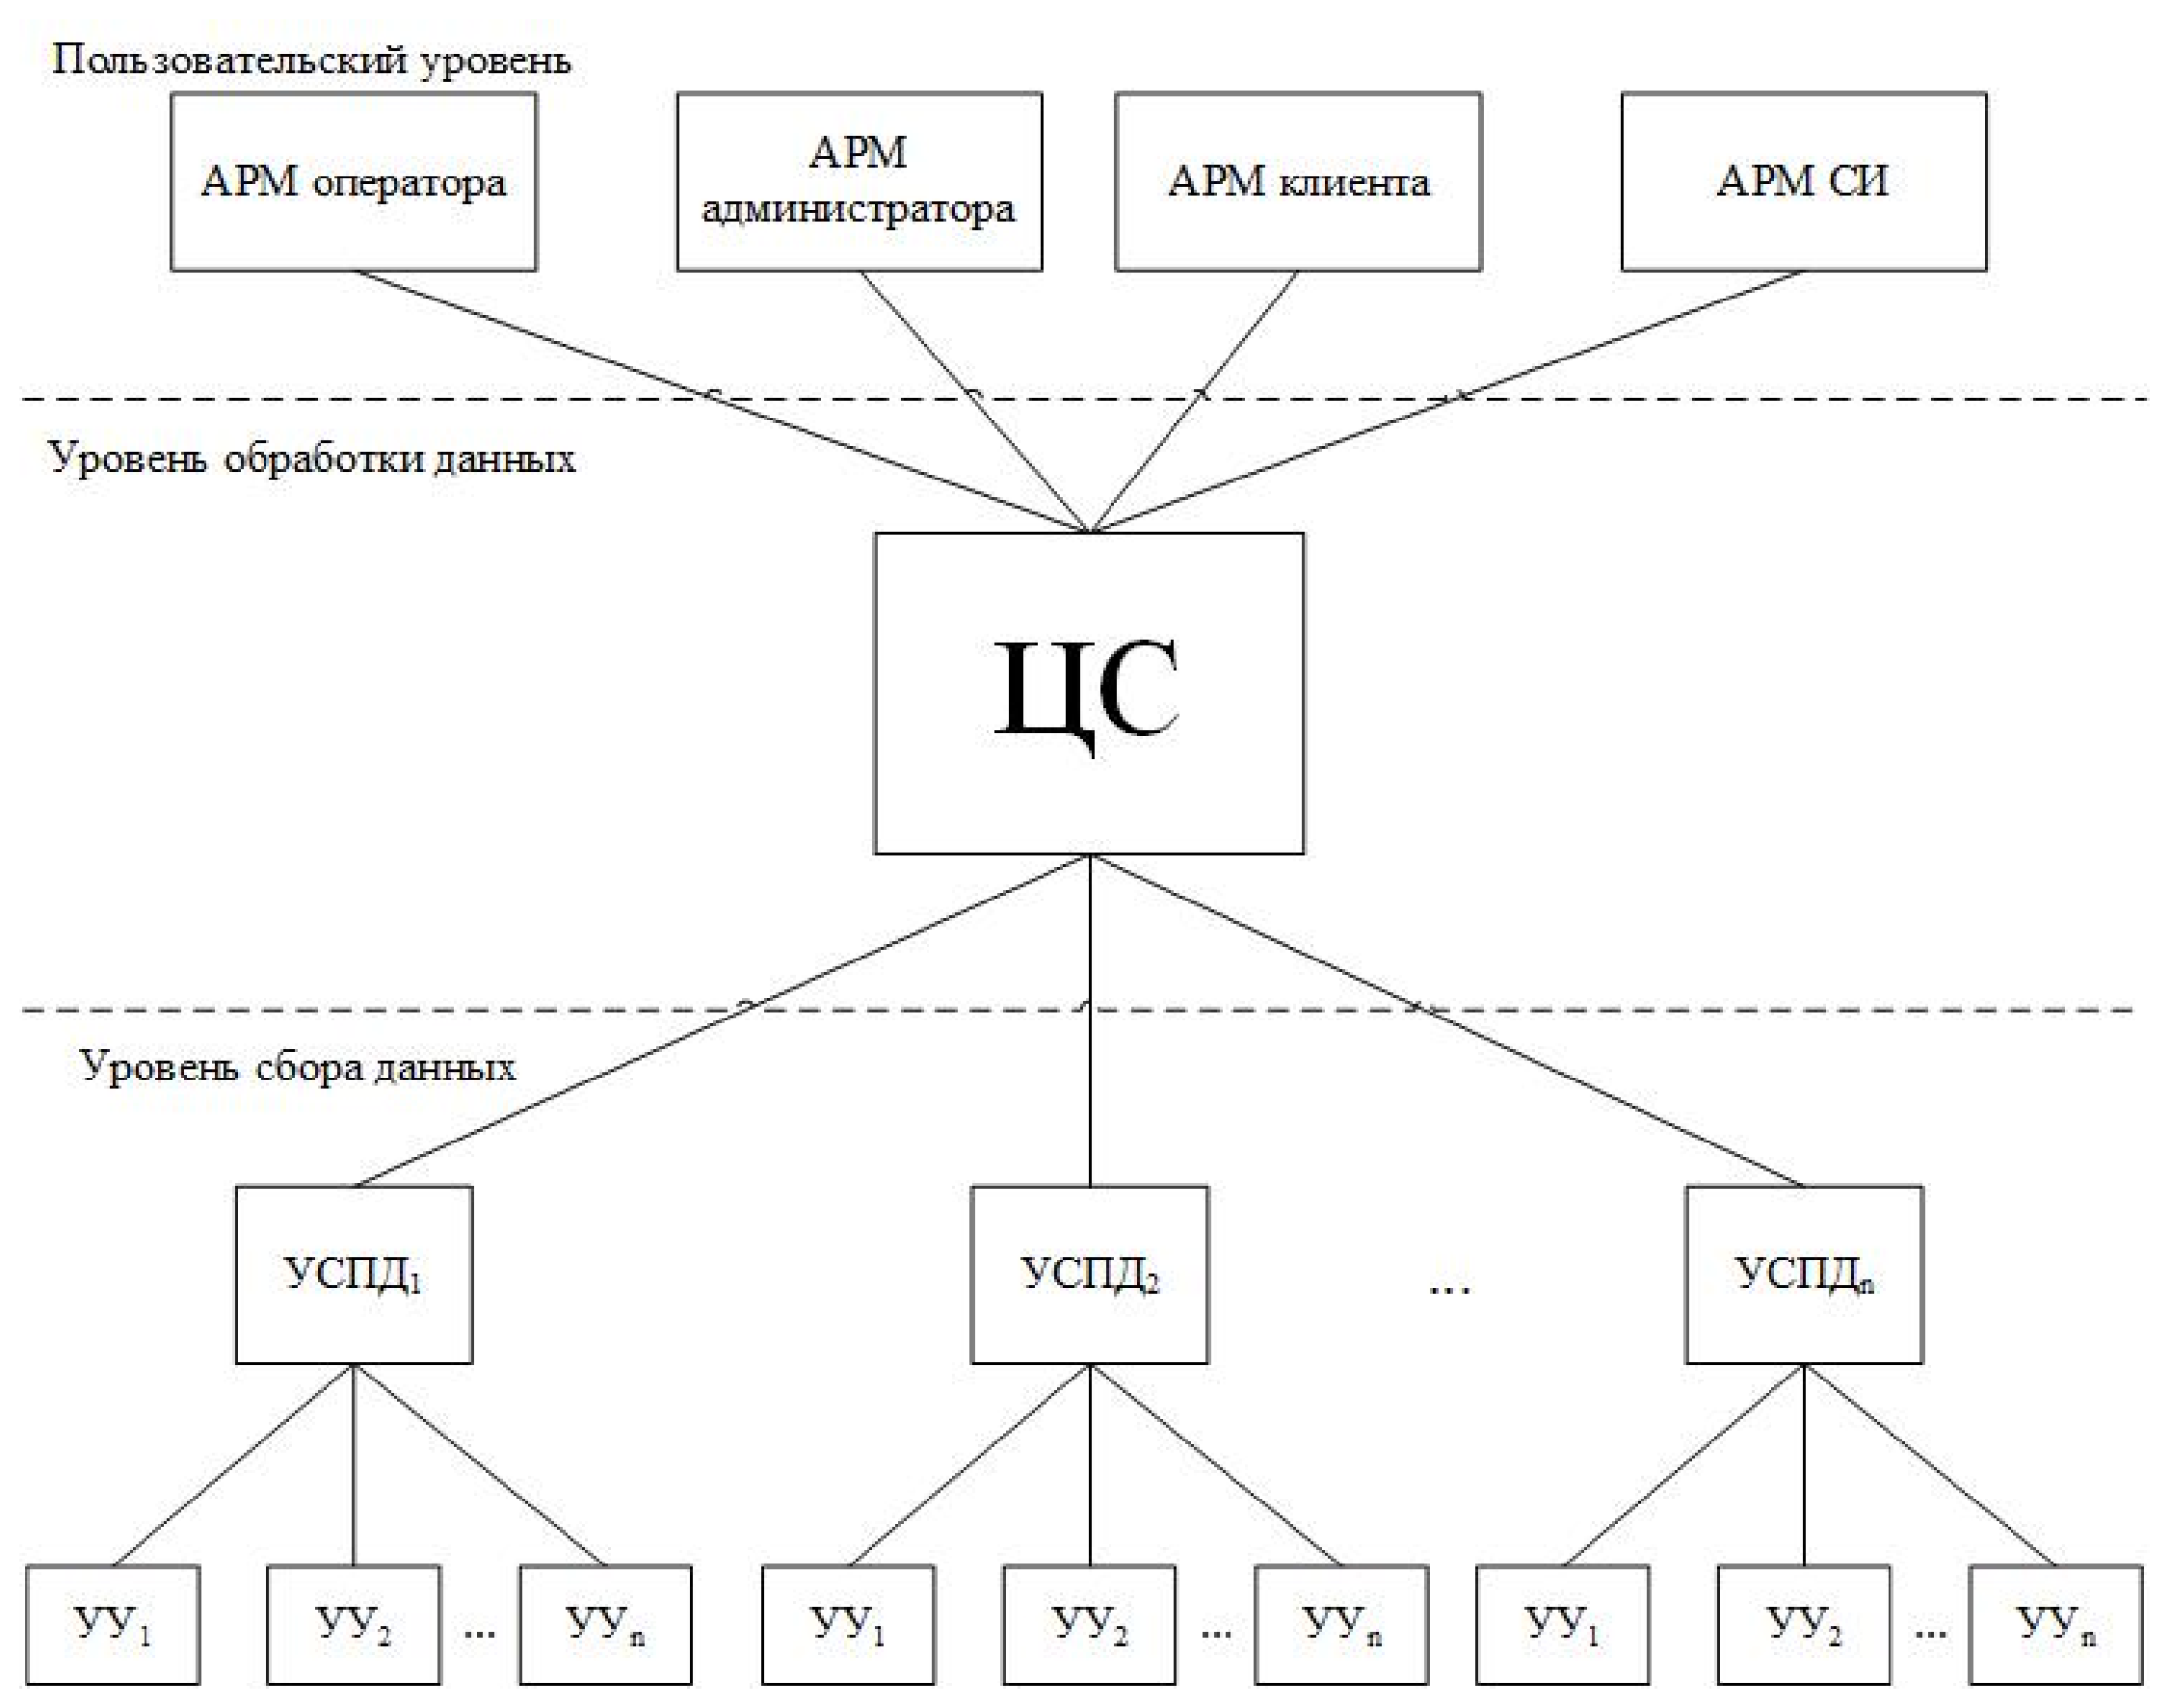
\includegraphics[width=0.8\linewidth]{irsh}}
 \caption{Структурная схема АСКУЭ}
 \label{irsh:irsh}
\end{figure}

\subsection{Описание сервера сбора данных}

ССД обслуживает низкоуровневое взаимодействие с УСПД. После получения данных этот блок передает информацию модульной системе драйверов. Система драйверов осуществляет взаимодействие на верхнем уровне модели OSI. За счет модульности обеспечивается расширение парка поддерживаемого оборудования. Также ССД содержит систему управления сетью и взаимодействия с базой данных: он осуществляет контроль работоспособности сети, выполняет отбраковку данных, отвечает за принятие решений о повторном запросе на сбор данных, классифицирует информацию, обеспечивает контроль единого времени и осуществляет запись информации в базу данных.

Логически ПО ССД можно разделить на 3 блока, каждый из которых выполняет отдельную задачу:
\begin{enumerate}
\item блок контроля приема и передачи данных, который отвечает за взаимодействие ССД с УСПД/УУ;
\item временная база данных (ВБД). В ходе проектирования ПО ССД было рассмотрено два варианта обработки и записи данных с УСПД/УУ на СБД: 
\begin{itemize}
\item обработка и запись данных на СБД по мере их поступления от УСПД/УУ;
\item запись поступающих данных в ВБД и последующая обработка и передача на СБД.
\end{itemize}
\item блок обработки данных.
\end{enumerate}

Использование первого варианта может привести к потере данных, так как вновь поступающие данные не будут успевать обрабатываться ПО ССД. Второй вариант позволяет обеспечить целостность поступивших данных, поэтому он является более предпочтительным.

Обобщенная функциональная схема функционирования ПО ССД представлена на рисунке \ref{sh_ssd:sh_ssd}.

\begin{figure}[h!]
 \center{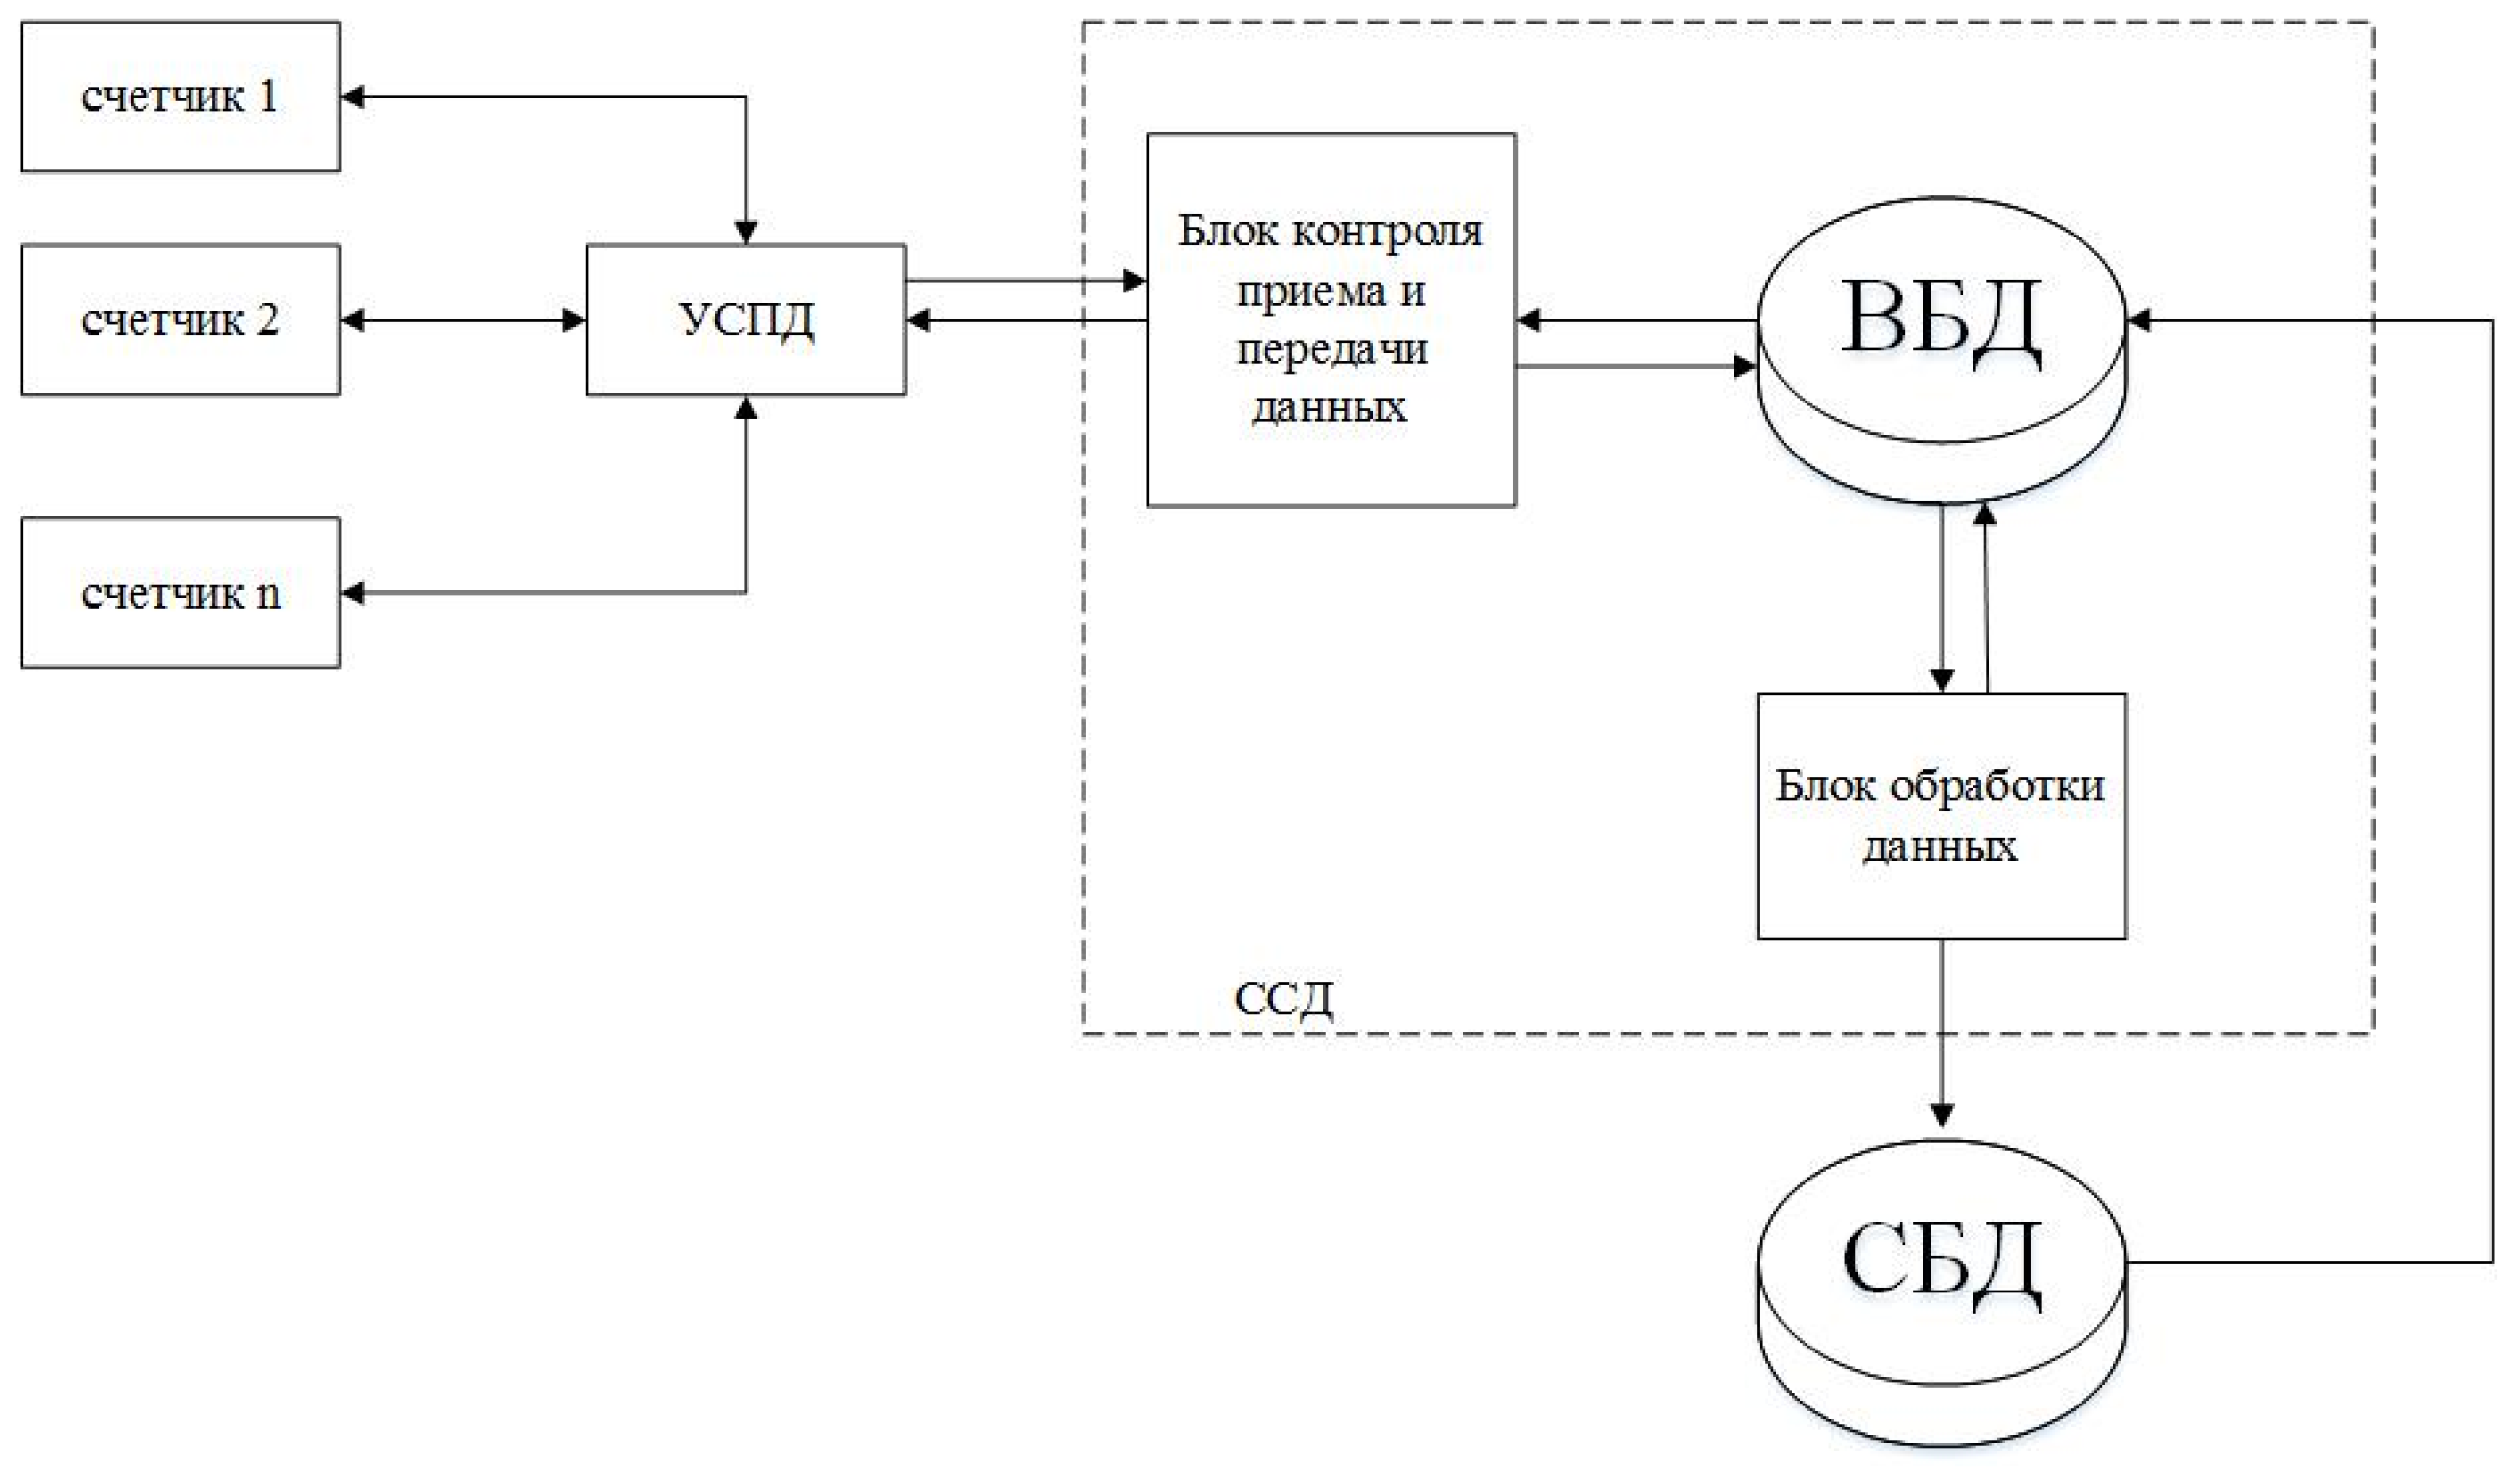
\includegraphics[width=0.8\linewidth]{sh_ssd}}
 \caption{Функциональная схема ССД}
 \label{sh_ssd:sh_ssd}
\end{figure}

%TODO
\begin{itemize}
 \item передача данных по Кококоналам связи;
 \item контроль потоков инфлрмации;
 \item Конфиденциальность;
 \item целостность Данных.
\end{itemize}

\subsection{Описание устройства съема и передачи данных}

Устройство съема и передачи данных является промежуточным звеном между устройствами учета и сервером сбора данных. Оно предназначено для непосредственного управления устройствами учета, их опроса, настройки и диагностики. Всю инофрмацию от устройств учета и о их состоянии ССД получает от УСПД.

%TODO
\begin{itemize}
 \item контроль подключений;
 \item идентификация, аутентификация;
 \item хзчоещё
\end{itemize}